\documentclass[12pt,a4paper]{report}

\begin{document}
%titel
\title{DIA}
\author{Ward Pennemans - 2TinH}
\maketitle
%titel

\begin{flushleft}

Dit document is geschreven met behulp van \LaTeX{} wat geen programma is, maar een reeks macro's. Om deze tekst te schrijven en te compileren wordt er gebruik gemaakt van de programma's Texmaker en MiKTeX.

\newpage

%-----Begin Inhoud-----
\begin{center}
\begin{LARGE}
\textbf{Inhoud}
\end{LARGE}		
\end{center}
\begin{enumerate}
\item Wat is Dia?
\item Oorsprong
\item Waarom Dia gebruiken?
\item Waarom Dia niet gebruiken?
\item Installatie
\item Gebruik van Dia
\begin{enumerate}
\item Aanmaken van shapes
\item werken met Dia
\begin{enumerate}
\item Het werkveld
\item Werkbalk en diagrammen
\item Een diagram maken
\end{enumerate}
\end{enumerate}
\item versiebeheer
\end{enumerate}
%-----eind Inhoud-----

\newpage

%-----Begin Hoofdstuk Wat is Dia?-----
\chapter{Wat is DIA?}
\paragraph*{}
Dia is een gratis en open source applicatie om technische diagrammen te ontwikkelen, en kan objectief worden vergeleken met Visio van Microsoft. Het programma is gebaseerd op het GTK+ principe. GTK+ of GIMP Toolkit is een multiplatform werkset om gebruikersomgevingen te ontwerpen. Net zoals GTK+ is Dia geschreven in de programmeertaal C. 
\paragraph*{}
Op dit moment heeft Dia een aantal hulpmiddelen om de gewenste schema's eenvoudig te ontwerpen, nl. ERD-schema's(Entity Relationship Diagramà, UML diagrmmen, stroomdiagrammen, netwerkschema's, elektriciteitsschema's en andere. Een andere, zeer bruikbare eigenschap van Dia is dat het mogenlijk is om eenvoudig bestanden op te slaan als en te openen van een XML-document.
Omdat dia eenvoudig en vriendelijk is in gebruik, kunnen mensen met weinig ervaring er toch eenvoudig met werken. Toch is het programma ook flexibel en krachtig genoeg om de meer ervaren gebruikers toe te laten om zeer geavanceerde schema's te ontwerpen.
\paragraph*{}
De laatste versie van Dia op dit moment is 0.97.2, beschikbaar sinds 18/12/2011. Deze versie is te downloaden op \textit{http://dia-installer.de/}.
%-----Eind Hoofdstuk Wat is Dia?-----

%-----Begin Hoofdstuk Oorsprong-----
\chapter*{Oorsprong}
Dia is ontwikkeld door Alexander Larsson . Hij stopte met het ontwikkelen van Dia en stapte over naar GNOME en andere projecten. Ook zijn opvolger, James Henstridge ging over tot het werken met andere projecten. Hierna werden Cyrille Chepelov en Lars Raeder Clausen hoofd van ontwikkeling van Dia. Het programma wordt onderhouden door een groep van software ontwikkelaars, DIA developers, die bestaat uit Hans Breuer, Steffen Macke en Sameer Sahasrabuddhe.
%-----Begin Hoofdstuk Oorsprong-----

%-----Begin Hoofdstuk Waarom Dia Gebruiken-----
\chapter*{Waarom DIA gebruiken}
\paragraph*{}
Dia is een open source software. Hierdoor is het een zeer flexibel programma dat voldoet aan de eisen van verschillende gebruikers. Het grootste voordeel ten opzichte van concurrenten zoals Visio is echter dat het een gratis software is. Dia maakt gebruik van single document interface, d.w.z. dat er voor elk schema een nieuw venster wordt geopend. Dit kan zowel positief als negatief zijn. Voor een klein aantal projecten is het eenvoudig dat elk schema een apart venster heeft met een eigen toolbar. Echter indien er tegelijk aan een groot aantal schema's wordt gewerkt, zijn er vele vensters geopend waardoor het onoverzichtelijk kan worden. In de nieuwste versies van dia wordt ondertussen geen gebruik meer gemaakt van single document interface, maar van tabbladen.
\paragraph*{}
Doordat documenten, aangemaakt in Dia worden opgeslagen als XML-documenten, kunnen in Dia eenvoudig nieuwe vormen worden aangemaakt door te werken met een deelverzameling van Scalable Vector Graphics (SVG) en de gemaakte schema's kunnen door verscheidene andere programma's worden gelezen en aangepast. De schema's kunnen zelfs met de hand worden aangepast.
\paragraph*{}
Een ander voordeel dat voortkomt uit het gebruik van XML-documenten, is dat de schema's minder geheugen vereisen. Verder kunnen ook grotere schema's van meerdere pagina's worden opgeslagen.
\paragraph*{}
Dia kan bestanden opslaan en openen vanuit verscheidene formaten:
\begin{enumerate}
\item \textbf{EPS} (Encapsulated PostScript) Een grafisch bestand in de taal PostScript. Gebruikt door Adobe Photoshop en Adobe Illustrator.
\item \textbf{SVG} (Scalable Vector Graphics) Een op XML gebaseerd bestandsformaat voor statische en dynamische vectorafbeeldingen. Het is aangeraden door W3C en is te vergelijken met Flash.
\item \textbf{DXF} (Drawing Interchange format) Een bestandsformaat van CAD om gegevens te kunnen uitwisselen tussen AutoCAD(een programma voor het ontwerpen van technische tekeningen, zowel 2D als 3D) en andere programma's.
\item \textbf{CGM} (Computer Graphics Metafile) Een internationaal gestandariseerd bestandsformaat voor 2D vectorgrafieken, rastergrafieken en text. Het is opgesteld door ISO/IEC.
\item \textbf{WMF} (Windows Meta File) Een grafisch bestandsformaat gebruikt in windowssystemen.
\item \textbf{PNG} (Portable Network Graphics) Een bestandsformaat voor rasterafbeeldingen met verliesloze compressie. 
\item \textbf{JPEG} (Joint Photographic Experts Group) Een bastandsformaat voor het opslaan van rasterafbeeldingen in digitaal formaat.
\item \textbf{VDX} Een bestandsformaat van Windows dat kan worden vergeleken met XML. Dit formaat wordt gebruikt voor Visio.
\end{enumerate}
%-----Eind Hoofdstuk Waarom Dia gebruiken-----


%-----Begin Hoofdstuk Waarom Dia niet gebruiken-----
\chapter*{Waarom DIA niet gebruiken}
Dia is niet zo geavanceerd, krachtig en visueel uitgewerkt als andere programma's om diagrammen te ontwerpen zoals Visual Paradigm,... Toch is het voor de meeste gebruikers ruim voldoende door het grote aantal sets van vormen om verschillende diagrammen te ontwerpen en de mogelijkheid om er zelf te ontwerpen. De pictogrammen waaruit een schema in Dia bestaat zijn niet zomaar figuren, ze hebben veel extra informatie. Hierdoor wordt het moelijk om zelf pictogrammen te ontwerpen. De schema's die men kan ontwerpen in Dia zijn niet heel visueel. gebruikers die een beter ogend diagram willen kunnen best het schema ontwerpen in Dia en daarna met een programma zoals Inkscape bewerken. Een laatste belangrijk nadeel aan het gebruik van Dia is dat er relatief weinig updates vrijkomen. Echter omdat er zelf pictogrammen kunnen worden aangemaakt en aangezien het programma open source is kunnen de meer geavanceerde gebruikers (met kennis van C en XML) zeker vlot verder.
%-----Eind Hoofdstuk Waarom Dia niet gebruiken-----


%-----Begin Hoofdstuk Installatie-----
\chapter*{Installatie}
Download één van de volgende bestanden:
\linebreak\linebreak
\textbf{Ubuntu} (\textit{http://dia-installer.de/})\linebreak
In Ubuntu is Dia ook simpelweg te installeren via het ubuntu software center.
\linebreak\linebreak
\textbf{Windows} (\textit{http://dia-installer.de/})\linebreak
De source packages zijn te downloaden van \textit{http://ftp.gnome.org/pub/gnome/sources/dia/}
\linebreak\linebreak
\textbf{Mac} (\textit{http://dia-installer.de/})\linebreak
De source packages zijn te downloaden van \textit{http://ftp.gnome.org/pub/gnome/sources/dia/}
%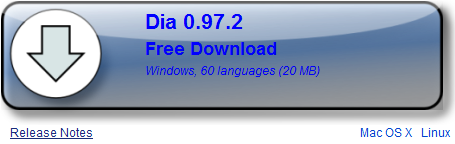
\includegraphics[scale=1]{install_01.png}
\linebreak\linebreak
Volg de wizard die hierna wordt geopend.
%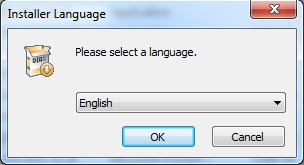
\includegraphics[scale=1]{install_02.png}
%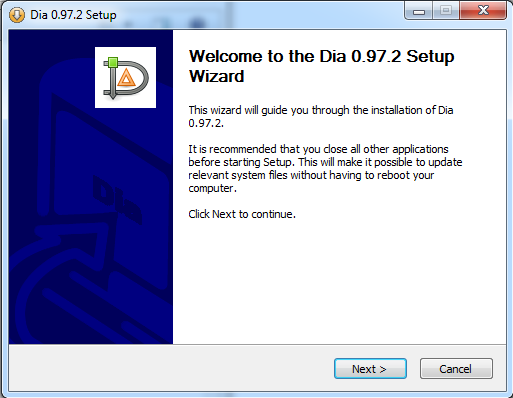
\includegraphics[scale=1]{install_03.png}
%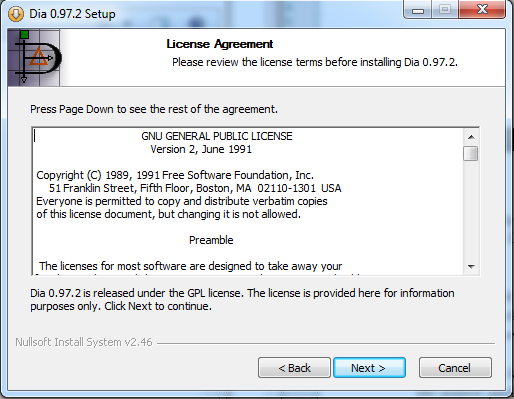
\includegraphics[scale=1]{install_04.png}
%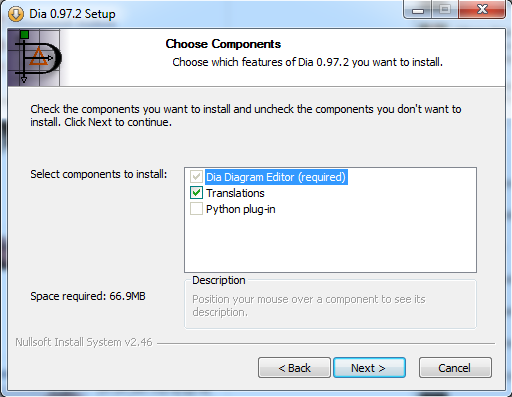
\includegraphics[scale=1]{install_05.png}
%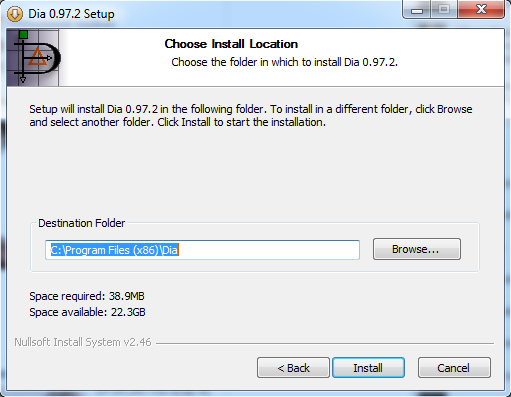
\includegraphics[scale=1]{install_06.png}
%-----Eind Hoofdstuk Installatie-----


%-----Begin Hoofdstuk Gebruik van Dia-----
\chapter*{Gebruik van Dia}
%-----Begin sectie Aanmaken van shapes-----
\subsection*{Aanmaken van shapes}
Er zijn 2 manieren om een vorm aan te maken in Dia.
\paragraph*{1}
De meest eenvoudige manier vergt geen kennis van XML of eenderwelk andere computertaal. Hierbij kan echter enkel een vorm worden gemaakt door verschillende bestaande vormen samen te voegen.
\paragraph*{}
Maak de gewenste vorm door verschillende vormen te slepen uit de toolbox. Ga vervolgens in het navigatiemenu bovenaan naar File/Export. Kies in het volgende venster het bestandstype Dia Shape File (*.shape). In het scherm dat u nu ziet, moet u de gewenste grootte van de vorm ingeven. 
\linebreak
%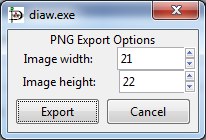
\includegraphics[scale=1]{shape_01.png}
\linebreak\linebreak
Druk vervolgens op Export. De vorm is beschikbaar.
\paragraph*{}
Om de vorm toe te voegen aan een diagram gaat u via het navigatiemenu naar File/Sheets and Objects. In dit vester kiest u in het linker drop-down menu de optie "Civil".
\linebreak
%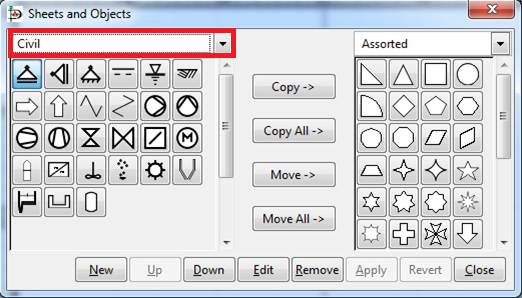
\includegraphics[scale=1]{shape_02.png}
\linebreak
Om de vorm toe te voegen klikt u op de knop "New". In het volgende scherm moet u het pad ingeven van het .shape file. Dit doet u best via de knop "Browse".
\linebreak
%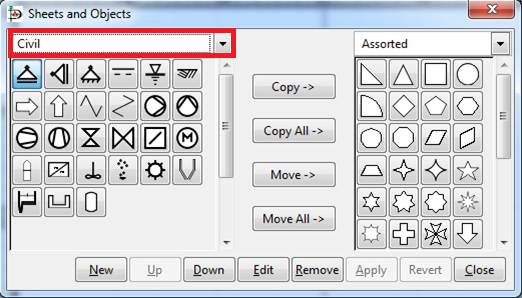
\includegraphics[scale=1]{shape_02.png}
\linebreak
 In het tekstvak description geeft u een beschrijving van het object in. Klik op "OK" en de vorm is toegevoegd aan het Civil menu.

\paragraph*{2}
De tweede manier vergt enige kennis van XML-code. 
Maak een bestand aan met notepad, wordpad of een ander tekstbewerkingsprogramma.
Voer een reeks code in zoals hieronder.
\linebreak
%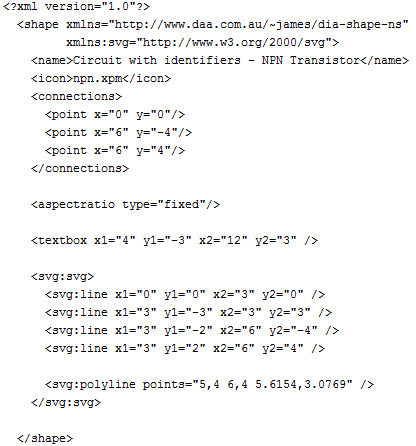
\includegraphics[scale=1]{shape_04.png}
\linebreak
Sla dit document op als een *.shape file. Doorloop nu de stappen van de eerste manier om de vorm toe te voegen aan Dia.
%-----Eind sectie Aanmaken van shapes-----

%-----Begin sectie Werken met Dia-----
\subsection*{Werken met Dia}
\subsubsection*{Het werkveld}
%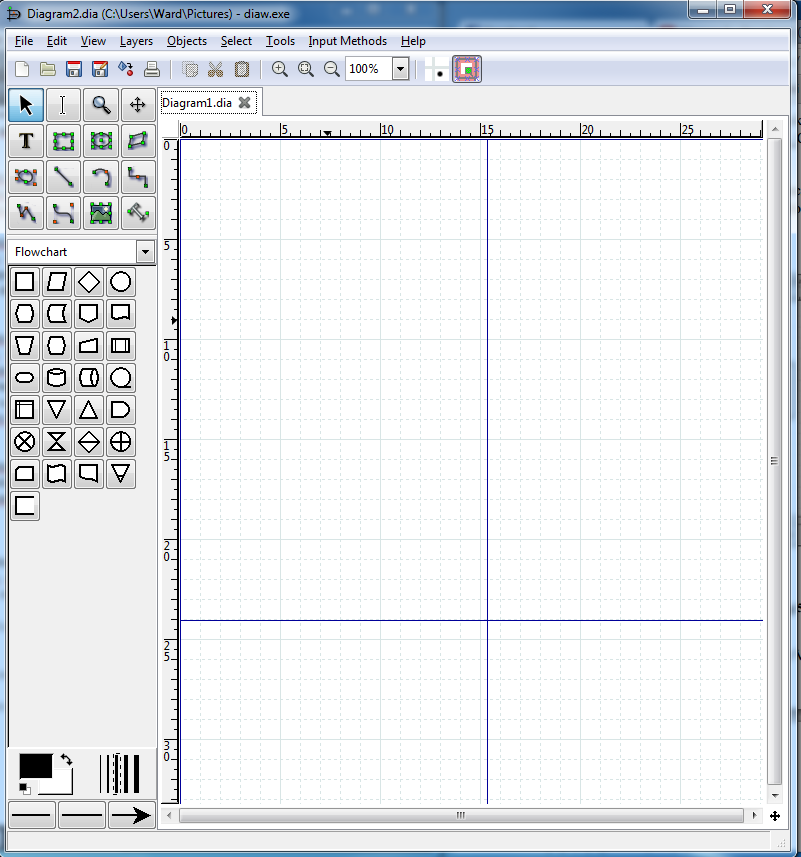
\includegraphics[scale=1]{werkveld_01.png}
%\linebreak
\paragraph*{}
Bovenaan vindt u zoals bij elke applicatie de standaard menubalk met daaronder een menubalk van DIA zelf. Links in het venster staat de werkbalk met de diagrammen in een drop down menu zoals de afbeelding hieronder laat zien. Rechts van de werkbalk bevind zich het echte werkveld waarin u het diagram zal plaatsen.
\linebreak
%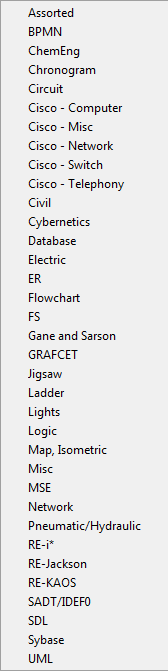
\includegraphics[scale=1]{werkveld_02.png}

\subsubsection*{Een diagram maken}
\paragraph*{}
Een diagram maken in Dia is zeer eenvoudig aangezien alle symbolen in de werkbalk staan. U moet enkel naar het juiste item in het drop-down menu navigeren voor de juiste symbolen. Hieronder enkele voorbeelden van diagrammen, gemaakt in Dia.
%-----Eind sectie Werken met Dia-----
%-----Eind Hoofdstuk Gebruik van Dia-----

\chapter{Versiebeheer}
\paragraph*{}
Voor de versiebeheer is er gebruik gemaakt van het programma GIT, te downloaden van http://git-scm.com/downloads.
\paragraph*{}
Git is een vrij gedistribueerd versiebeheersysteem. Het is gemaakt voor de ontwikkeling van de linuxkernel door Linus Torvalds. Iedere GIT werkmap bevat de volledige repository met een compleet historisch overzicht en volledige tracking capaciteiten. In tegenstelling tot CVS of SVN, concurrenten op het gebied van versiebeheer, is GIT niet afhankelijk van een gemeenschappelijke locatie of een centrale server.
\paragraph*{}
In dit document is gebruik gemaakt van een repository server van github, al is dit niet nodig en kan het ook locaal worden toegepast.
Op \textit{http://help.github.com/win-set-up-git/} is een zeer goede tutorial te vinden voor het installeren en gebruiken van GIT en Github.
\section*{Aanpassen van de github-directory}
Voor het toevoegen, bewerken of verwijderen van een bestand moeten een aantal stappen worden doorlopen.
\paragraph*{1}
Indien u een bestand wil toevoegen, moet u ervoor Zorgen dat het bestand in de directory staat die u in de tutorial heeft aangemaakt.
\paragraph*{2}
Met het commando "git status" zal GIT zoeken naar wijzigingen in de aangeduide directory en deze tonen.
\paragraph*{3}
Om een bestand toe te voegen maakt u gebruik van het commando "git add \textit{NAAM VAN HET BESTAND}", om een bestand te verwijderen is het commando "git rm \emph{NAAM VAN HET BESTAND}" van toepassing.
%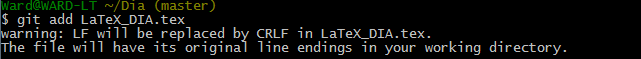
\includegraphics[scale=1]{../git_01.png} 
\paragraph*{4}
Vervolgens moet u het bestand committen door gebruik te maken van het commando "commit -m "\textit{TITEL VAN DE BEWERKING}""
%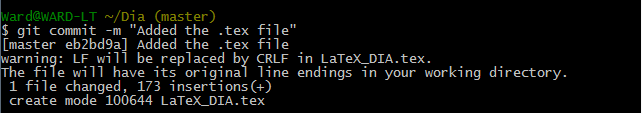
\includegraphics[scale=1]{../git_02.png} 
\paragraph*{4}
Ten slotte moet de wijziging worden doorgevoerd naar de github server. Dit doet u via het commando "git push origin master".
%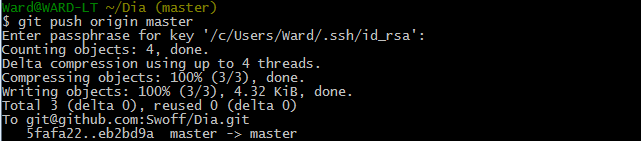
\includegraphics[scale=1]{../git_03.png} 
\end{flushleft}
\end{document}

